\subsection{Temperature and Salinity Changes}\label{sec:temp+sal}
To get a better picture of the changes that occur during the time periods we compare differences in sea temperature and salinity at 250m depth between the models. We do not use the sea surface temperature and salinity here because of the restoring boundary conditions used on the top layer of the ocean. It is important to note that these restoring boundary conditions with the simplified forcings make a discussion on the thermohaline circulation to be of limited value. But we can get an idea of what general changes occur. For a full overview of the salinity and temperature profiles the reader is referred to the appendices at the end of this paper.

First, we compare the differences between the 55Ma basin and the 35Ma basin (\cref{fig:5535cooling}). Here we see substantial differences between the two. One of the key features of the Eocene seems to be a large amount of cooling in the southern Atlantic along with a heating of the southern pacific. We also see that the Salinity changes closely match the locations of the Temperature increases. However, this is less noticeable in the northern Atlantic where the change in salinity is relatively smaller.


\begin{figure}[H]
	\begin{subfigure}[b]{\linewidth}
		\caption{}
		\label{fig:5535cooling}
		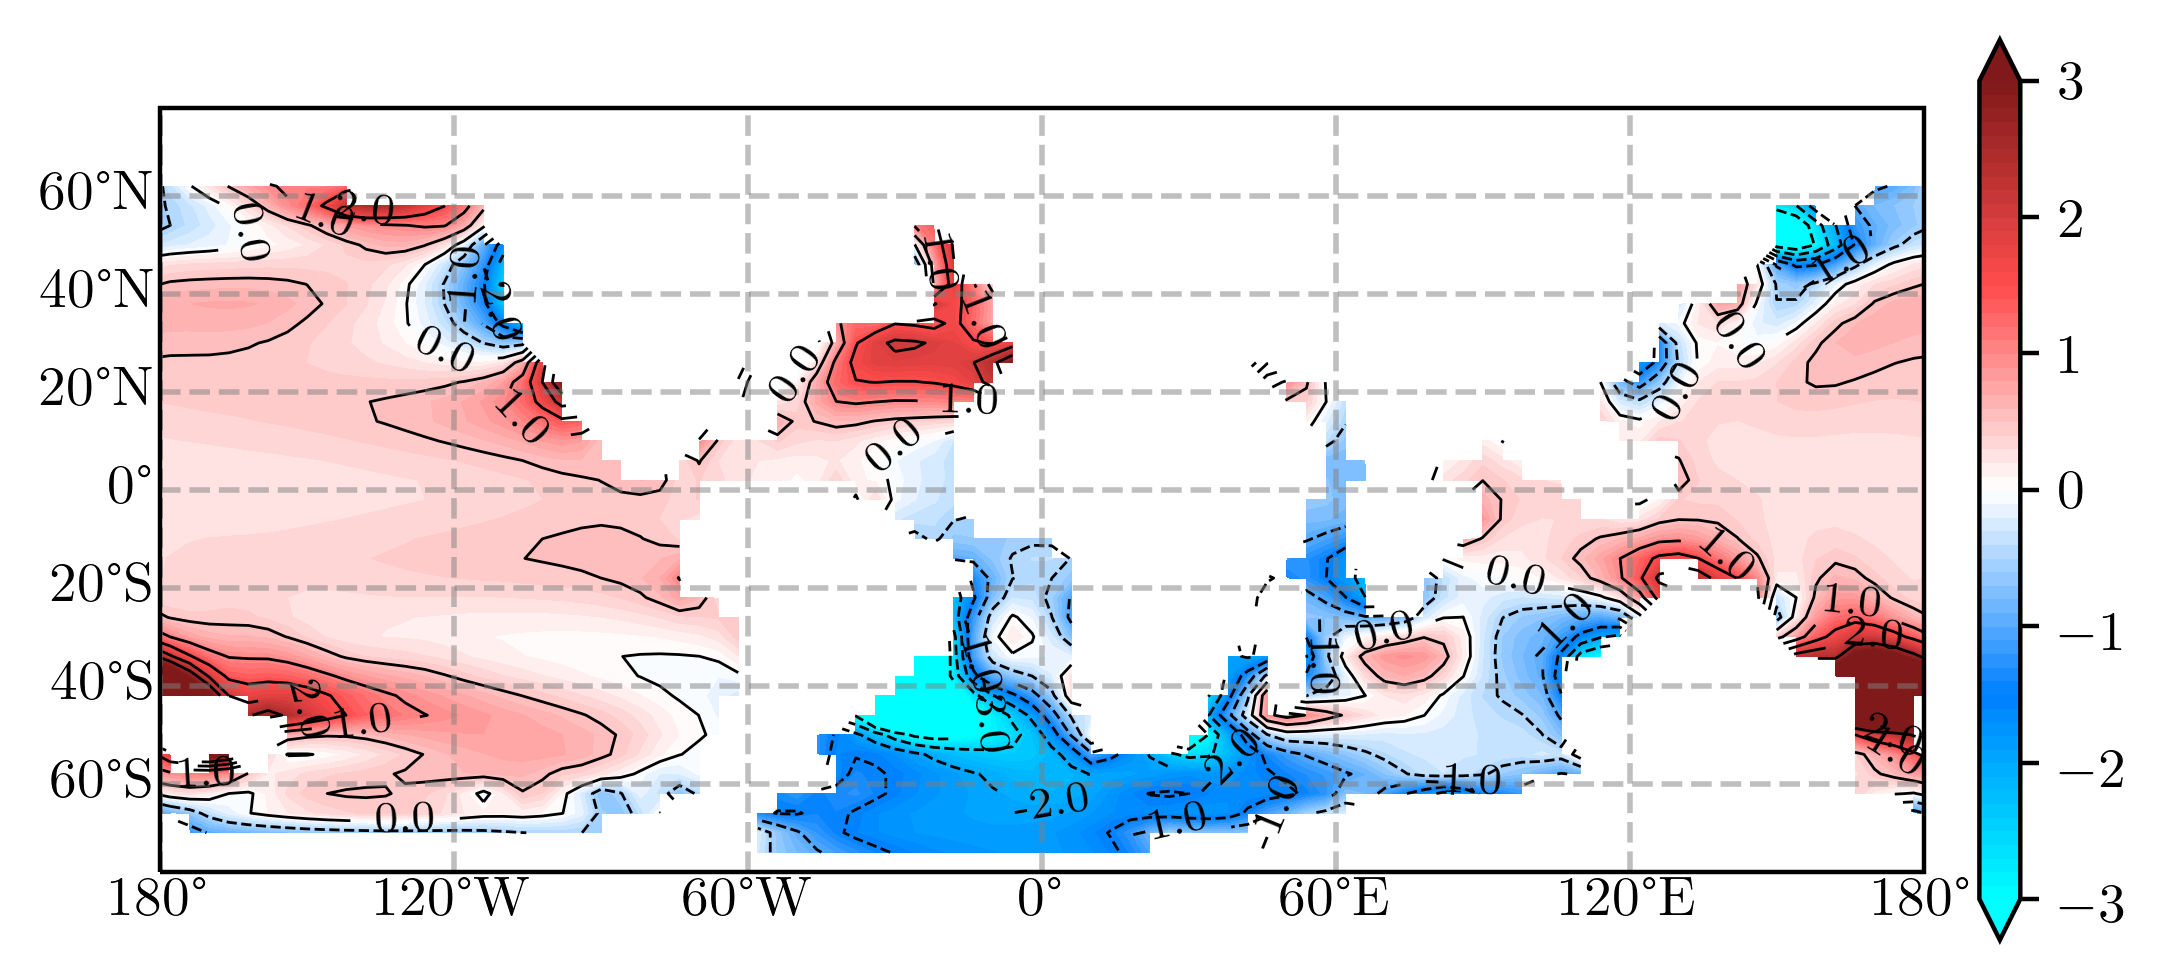
\includegraphics[width=\linewidth]{Paleo_eocene_55_35.png}
		
		
	\end{subfigure}
	\begin{subfigure}[b]{\linewidth}
		\caption{}
		\label{fig:salt5535cooling}
		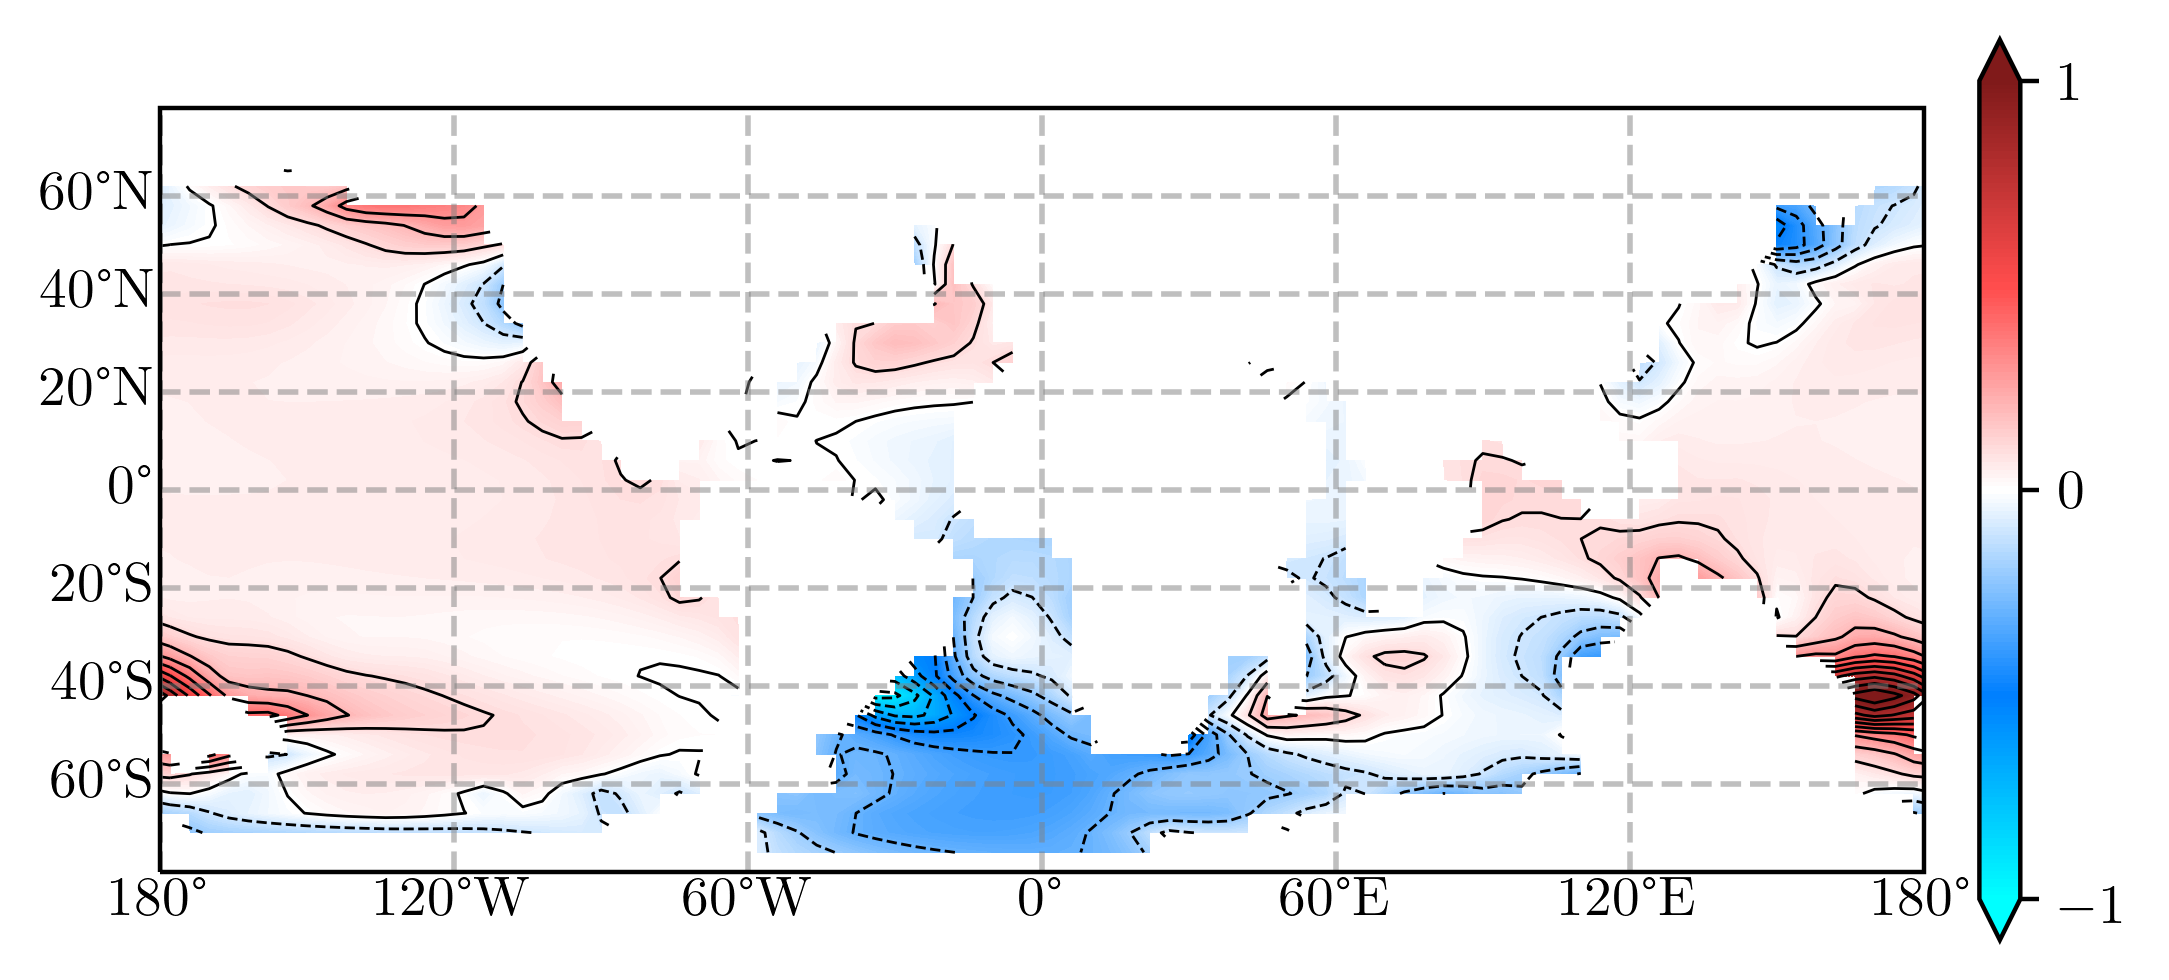
\includegraphics[width=\linewidth]{salt_55_35.png}
		
		
	\end{subfigure}
	\caption{ Comparison between late Paleocene (55Ma) and late Eocene (35Ma) for: \textbf{a)} Temperature ($^{\circ}C$) differences (positive values indicate warming) and  \textbf{b)} Salinity ($psu$) differences (positive values indicate higher salinity)}
\end{figure}

\begin{figure}[H]
	\begin{subfigure}[b]{\linewidth}
		\caption{}
		\label{fig:3520cooling}
		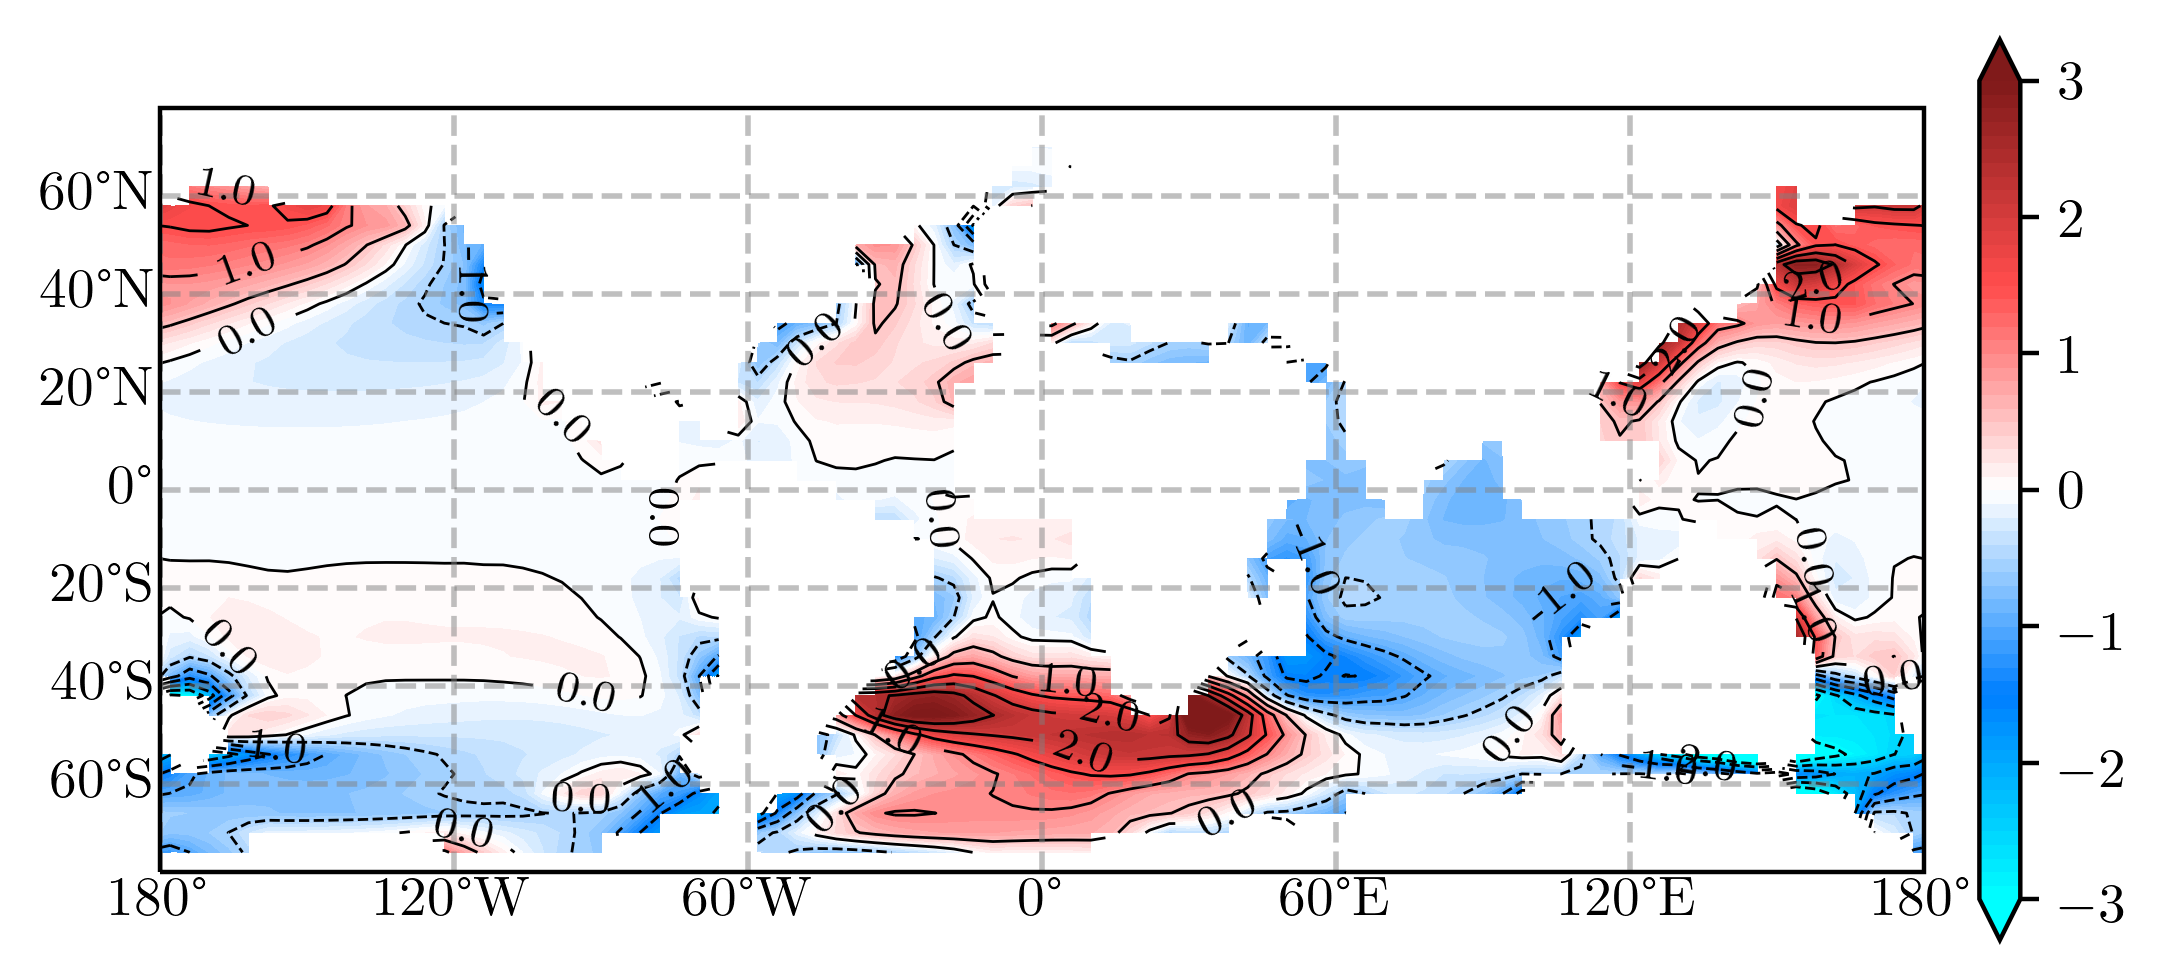
\includegraphics[width=\linewidth]{Paleo_eocene_35_20.png}
		
	\end{subfigure}
	\begin{subfigure}[b]{\linewidth}
		\caption{}
		\label{fig:salt3520cooling}
		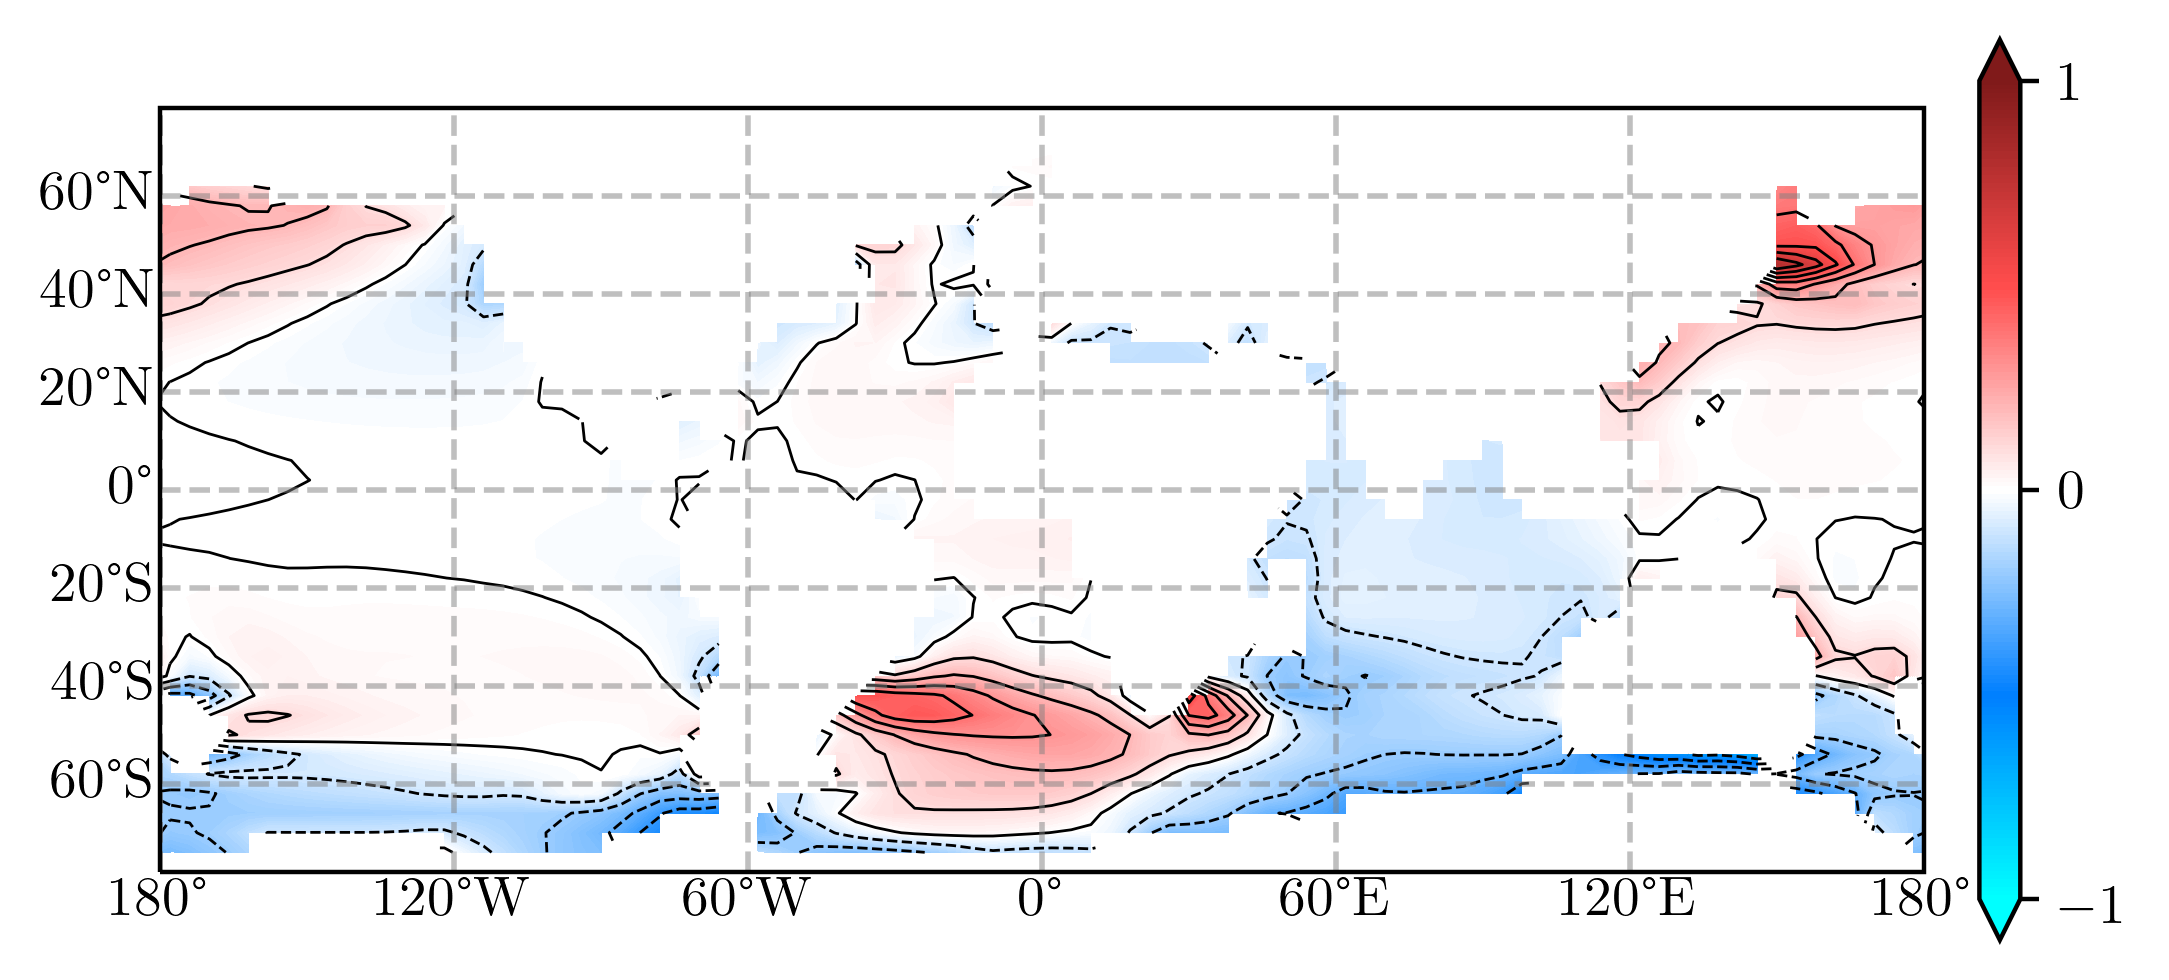
\includegraphics[width=\linewidth]{salt_35_20.png}
		
	\end{subfigure}
	\caption{ Comparison between late Eocene (35Ma) and early Miocene (20Ma) for: \textbf{a)} Temperature ($^{\circ}C$) differences (positive values indicate warming) and  \textbf{b)} Salinity ($psu$) differences (positive values indicate higher salinity)}
\end{figure}

\begin{figure}[H]
	\begin{subfigure}[b]{\linewidth}
		\caption{}
		\label{fig:2010cooling}
		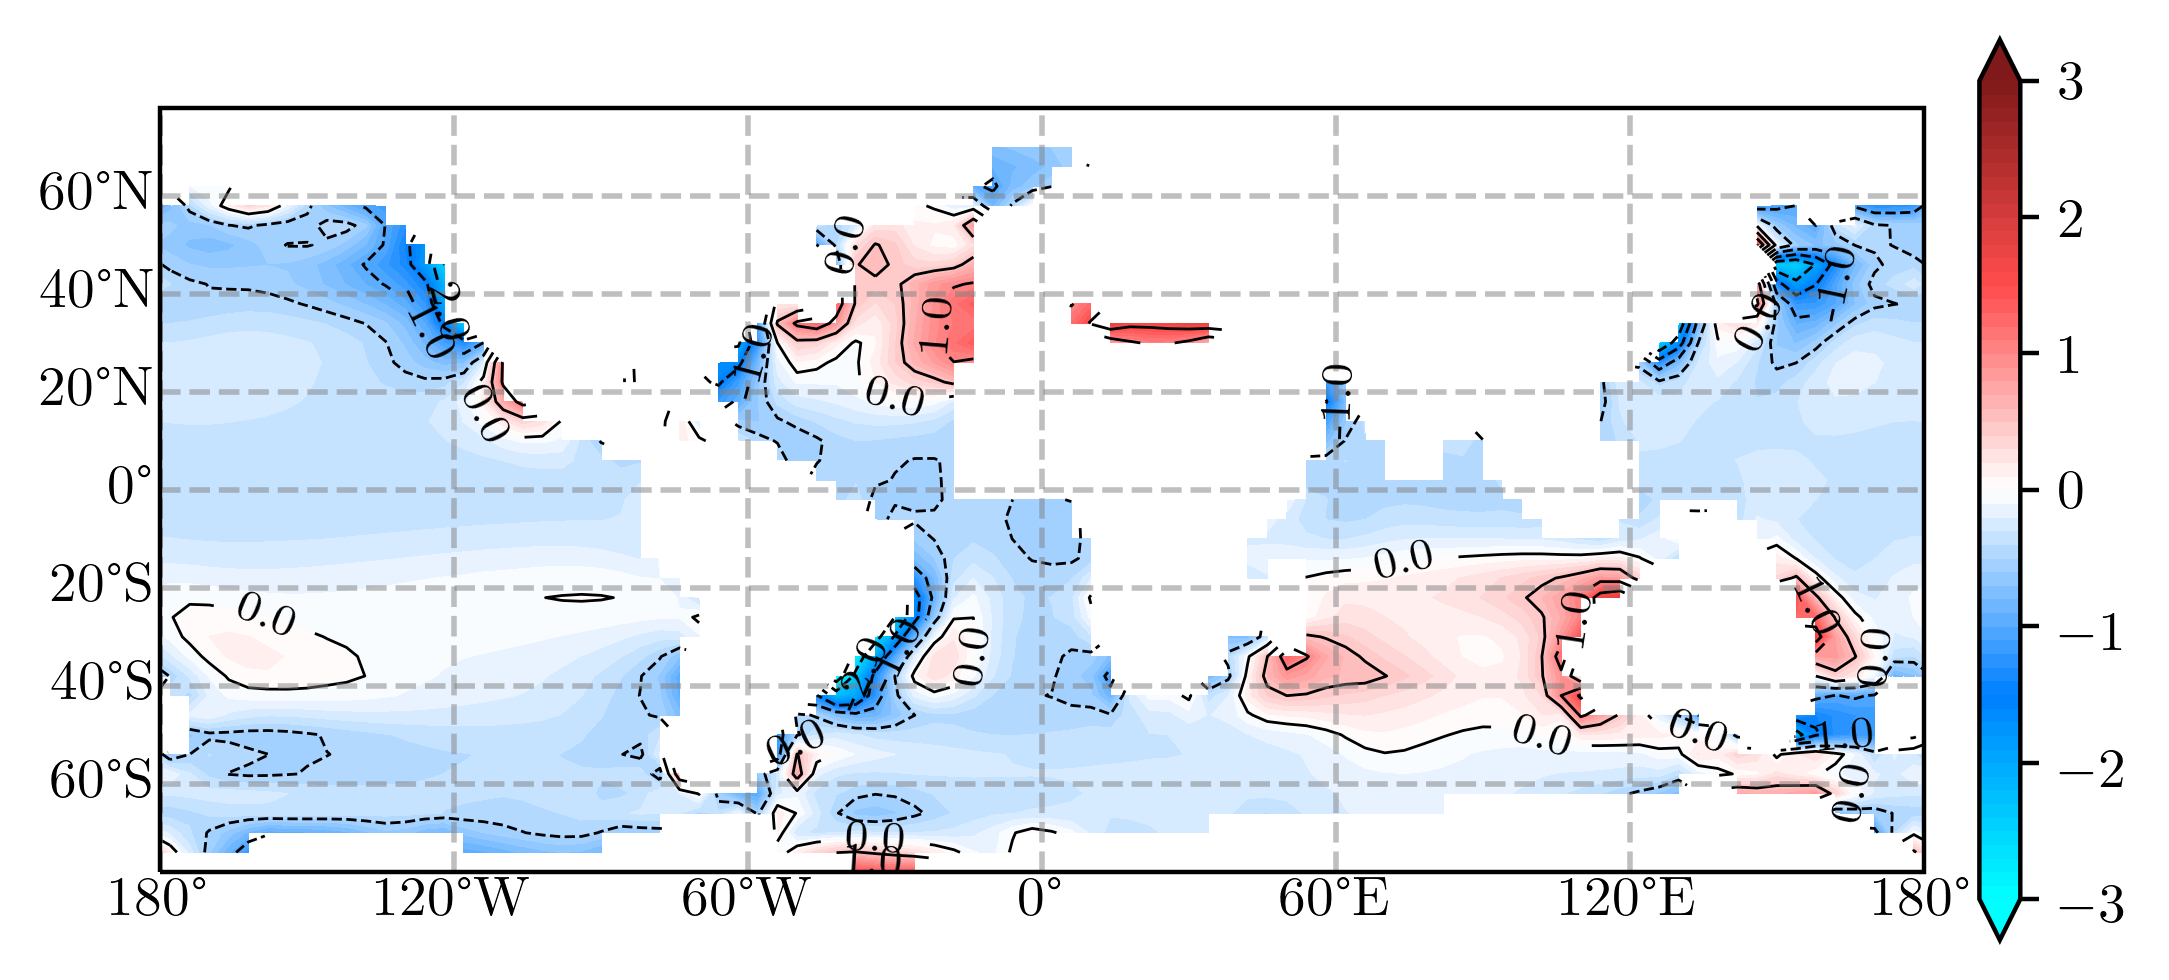
\includegraphics[width=\linewidth]{Paleo_eocene_20_10.png}
	\end{subfigure}
	\begin{subfigure}[b]{\linewidth}
		\caption{}
		\label{fig:salt2010cooling}
		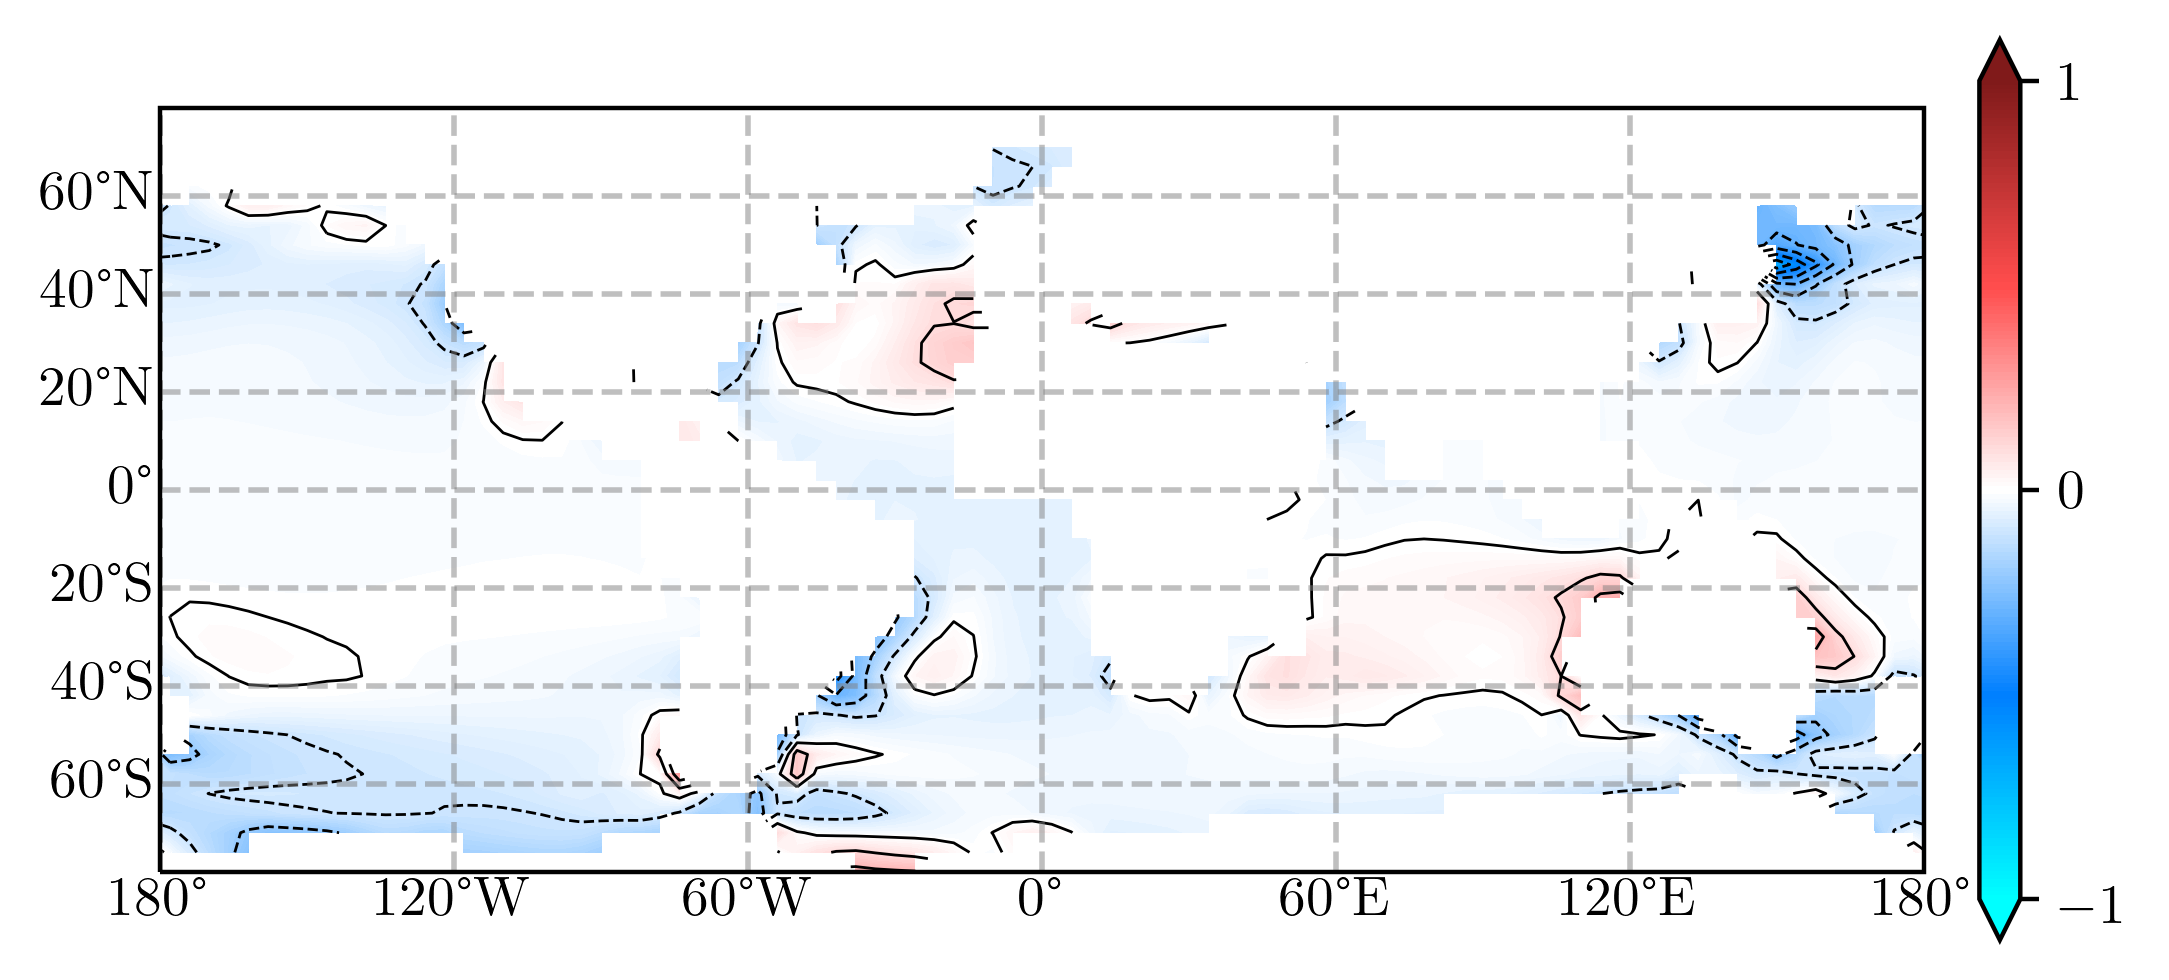
\includegraphics[width=\linewidth]{salt_20_10.png}
	\end{subfigure}
	\caption{ Comparison between early Miocene (20Ma) and late Miocene (10Ma) for: \textbf{a)} Temperature ($^{\circ}C$) differences (positive values indicate warming) and  \textbf{b)} Salinity ($psu$) differences (positive values indicate higher salinity)}
\end{figure}

